% Nikolai Nielsens "Fysiske Fag" preamble
\documentclass[a4paper,10pt]{article} 	% A4 papir, 10pt størrelse
\usepackage[english]{babel}
\usepackage{Nikolai} 					% Min hjemmelavede pakke
\usepackage[dvipsnames]{xcolor}

% Margen
\usepackage[margin=1in]{geometry}

% Max antal kolonner i en matrix. Default er 10
%\setcounter{MaxMatrixCols}{20}

% Hvor dybt skal kapitler labeles?
%\setcounter{secnumdepth}{4}	
%\setcounter{tocdepth}{4}


% Hvilket nummer skal der startes med i sections? (n-1)
%\setcounter{section}{0}	

% Til nummerering af ligninger. Så der står (afsnit.ligning) og ikke bare (ligning)
\numberwithin{equation}{section}


% Header
%\usepackage{fancyhdr}
%\head{}
%\pagestyle{fancy}

%Titel
\title{Numerical Methods in Physics Week 1}
\author{Nikolai Plambech Nielsen, LPK331. Version 1.0}
\date{\today}

\begin{document}
	\maketitle
	\section{Nuclear Decay}
	We have two radioactive isotopes, A and B, with populations $ N_A(t) $ and $ N_B(t) $, and decay times $ \tau_A $  and $ \tau_B $. Type A decays into type B, while B decays into something else we don't track. The relevant differential equations are
	\begin{equation}\label{key}
		\diff[\ud]{N_A}{t} = - \frac{N_A}{\tau_A}, \quad \diff[\ud]{N_B}{t} = \frac{N_A}{\tau_A} - \frac{N_B}{\tau_B}.
	\end{equation}
	The purpose of this assignment is to solve this problem numerically for a number of different conditions, using Euler integration. This method is used for its simplicity and ease of implementation.
	
	\subsection{Compare the numerical and analytical solutions}
	The analytical solutions are given in the assignment, and are as follows:
	\begin{align}
		N_A(t) &= N_A(0) \exp\pp{-\frac{t}{\tau_A}}, \\
		N_B(t) &= \begin{cases}
		N_B(0) \exp\pp{-\frac{t}{\tau_A}} + t \frac{N_A(0)}{\tau_A} \exp\pp{-\frac{t}{\tau_A}}, & \tau_A= \tau_B, \\
		N_B(0) \exp\pp{-\frac{t}{\tau_B}} + \frac{N_A(0)}{\frac{\tau_A}{\tau_B} - 1} \bb{\exp\pp{-\frac{t}{\tau_A}} - \exp\pp{-\frac{t}{\tau_B}}}, & \tau_A \neq \tau_B.
		\end{cases}
	\end{align}	
	The results, along with residual plots, for $ N_A(0) = N_B(0) = 1000 $ and $ \tau_A = 5, \tau_B = 10 $ are shown below:
	\begin{figure}[H]
		\centering
		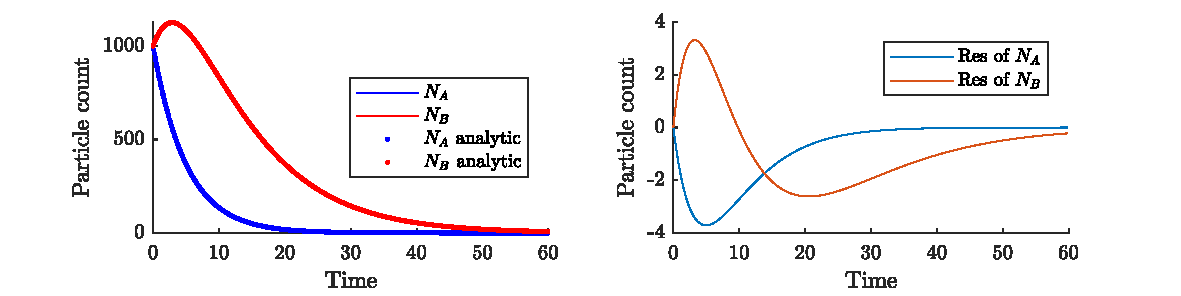
\includegraphics[width=0.7\linewidth]{unequaltau.pdf}
	\end{figure}
	
	
\end{document}

